\documentclass[letterpaper, 12pt]{article}
\usepackage{comment} % enables the use of multi-line comments (\ifx \fi) 
\usepackage{lipsum} %This package just generates Lorem Ipsum filler text. 
\usepackage{fullpage} % changes the margin
\usepackage{cite}
\usepackage{subfig}
\usepackage{graphicx}
\usepackage{wrapfig}
\usepackage{amsfonts}
\usepackage{float}

\linespread{1.15}
\graphicspath{ {images/} }


\begin{document}
%Header-Make sure you update this information!!!!
\noindent
\large\textbf{Carbon Storage Project} \hfill \textbf{Joshua Zweig} \\
\normalsize Carbon Storage \\
Prof. Lackner \hfill Spring 2016 \\

\begin{centering}
\textbf{Short Listing Saline Reservoirs for Potential Carbon Storage} \\
A Look at the Viability of Candidate Reservoirs in the United States through\\
Fuzzy c-Means Clustering\\
\end{centering}

\section*{Abstract}


\section{Introduction}
\subsection{Carbon Storage}
Scope to US bc available data


Motivation and whats what

\subsection{Potential Storage Site: Saline Formations}

\begin{wrapfigure}{r}{0.5\textwidth} %this figure will be at the right
    \centering
    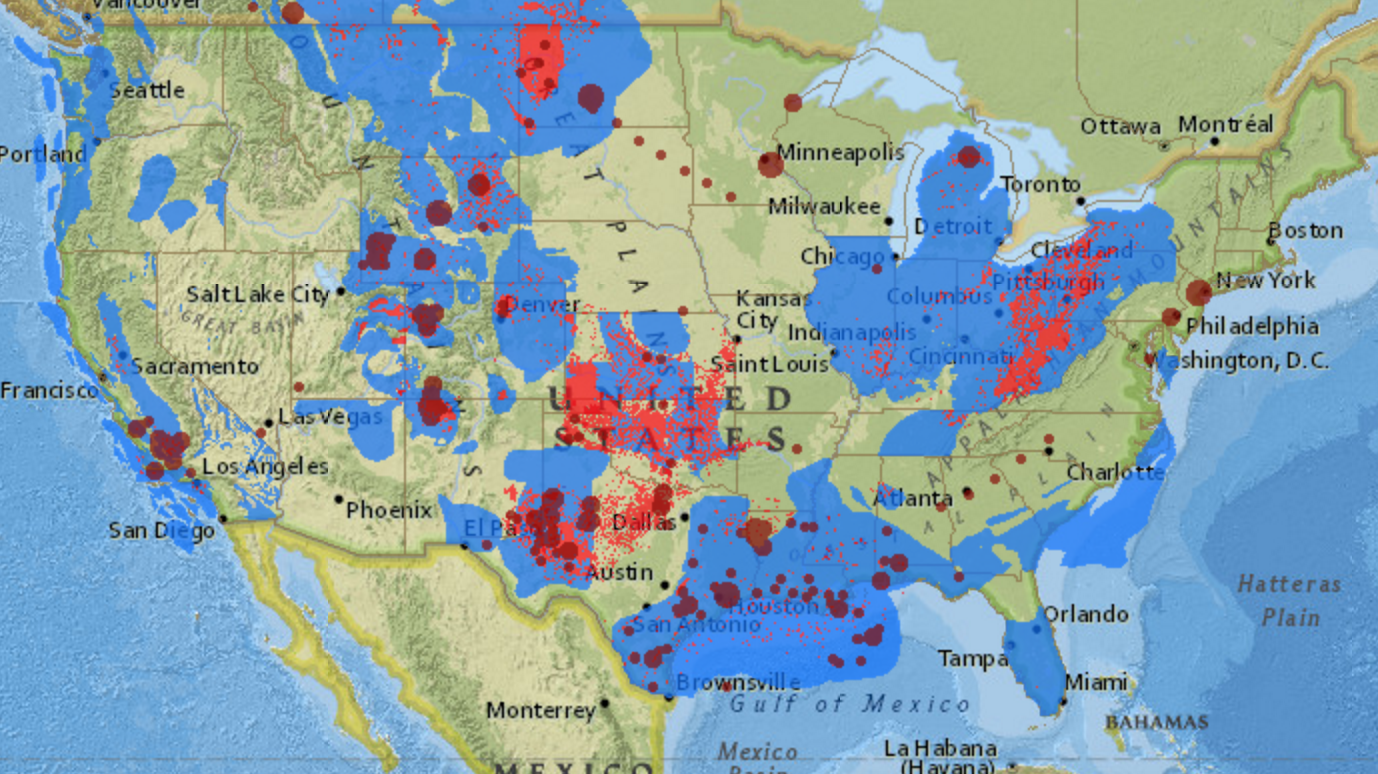
\includegraphics[width=0.5\textwidth]{saline_tight}
    \caption{\label{salinetight} A map of the United States overlaid with geological saline resources for potential carbon storage (blue), stationary sources of petroleum and natural gas (brown) and other oil and gas resources (red) \cite{atlas}.}
\end{wrapfigure}

\par Of possible candidates for long term carbon sequestration, saline formations have emerged as a promising candidate. Such formations are prevalent throughout North America. These brine coated layers of permeable rock are able to store carbon my way of "solubility trapping, mineral trapping, structural trapping and residual trapping."

The more than 180,000 potential injection sites in the United States have been estimated by the U.S. Department of Energy to have capacity of over 12 trillion tons of CO$_2$. Saline formations are promising also because of their proximity to CO$_2$ point sources, allowing easy transition of U.S. energy assets to "near-zero carbon emissions via low-cost carbon storage retrofits." \cite{whysaline} Furthermore, there is much existing technology and regulatory acceptance with respect to injections into saline reservoirs as brines are frequently injected into saline reservoirs in EOR and the U.S. EPA has designated some deep saline formations for hazardous waste disposal.

\par There are currently at least 3 saline aquifer injection projects that have been undertaken in the continental United States, which have together injected over a million tons of CO$_2$ to date. Each of these projects operates on a time scale of at least twenty years, allocating at least 10 years to "characterizing geologic and terrestrial opportunities for carbon storage and identifying CO$_2$ stationary sources within the territories of the individual RCSPs and evaluating promising CO$_2$ storage opportunities through a series of small-scale field projects"  \cite{midwestinject}, \cite{midwestinject2}, \cite{southeastinject}. 

Important Charecterists 



\subsubsection{Associated Risk} 
Maybe use that earthquake graph here....

\section{Methodology}
\subsection{Overview}
As described in the previous section, saline aquifers are luckily a far vast enough resource for us to currently store the desired amount of carbon. However, selecting the best aquifers for storage is a tremendous task considering the quantity of potential aquifers ($\approx180,000$) and the factors that characterize each one. For this reason we seek to develop a tool to immediately help identify some of the best candidate deep saline aquifers in the United States. 
The fundamental workings of this tool will be in the characterization of potential aquifers based on a series of characteristics as per section \ref{wellchar}. Having fully characterized each candidate aquifer, we fully employ a Fuzzy c-Means clustering analysis to each of the $\approx180,000$, 12 dimensional vectors representing the system to create a model that will determine how strongly each aquifer is characterized by each of the 12 features, to be discusses further in section \ref{fuzz}. Once this model is created, it will allow researchers to essentially filter potential storage sites by different characteristics and determine the relative similarity of unique sets of sites. For example, we will be able to observe all aquifers that have at least a given storage capacity and/or are at least a given distance from a major fault line.  

\noindent \emph{N.B. For the code that produced the results of this study, please see the repository \\at} https://github.com/joshuazweig/Carbon-Storage-Reservoir-Ranker \emph{where you can download the code and the data and run it yourself}

\subsection{Saline Aquifer Characterization} \label{wellchar}
Each of the 12 characterization dimensions falls into one of two categories. The first category of features describes the geological aspects of the formation, strictly its ability to store carbon. The second describes some of the factors that effect the potential risks and barriers to societal acceptance regarding potential storage sights.

\subsubsection{Geological Characterization}
The data regarding the geological characterization of the formations is from the data set "NATCARB Saline 10K, ver. 1502)" provided by the NATCARB project at the National Energy Technology Laboratory. The data primarily contains information on formations in the United States, which is the primary reason that this work is limited in scope the formations in the U.S. The dimensions included in the data set that will be combined with the data from the next section are \cite{atlas}: 
\begin{itemize}
\item \emph{Avg Volume/Capacity Estimate} Best estimate of storage capacity in metric tons. 
\item \emph {Depth} The mean depth in feet of the resource
\item \emph{Thickness}
\item \emph{Salinity} Mean salinity (total dissolved solids) of the resource
\item \emph{Pressure} Mean pressure in PPI of the formation
\item \emph{Temperature} Mean temperature in degrees Fahrenheit of the resource 
\item \emph{Porosity} Mean porosity percentage of the formation
\item \emph{Permeability} Mean permeability in millidarcies
\item \emph{Area, Longitude and Latitude} Given by the GIS shape file
\end{itemize}

\subsubsection{non-Geological Characterization}

The list below is a list of dimensions used to characterize saline formations with respect to environmental features not directly related to the ability of the formation to store carbon.
They are listed with reasonings for their inclusion in this early stage work in no particular order. As discussed in subsection \ref{betterchar}, this is a preliminary set of features I am considering for their importance and readily available data, but this by no means form an exhaustive list of relevant features of an injection site. The collection is meant to characterize storage potentials of saline formations, and for that reason I regard the dimension of the data set to be complete in this regard \cite{atlas}.

\begin{enumerate}
\item \emph{Potential Impact on Drinking Water Sources} It comes as no surprise that the proximity of a potential injection site to an important source of drinking water is important in considering the site's viability.  This notion is affirmed by the application of the Safe Drinking Water Act's Underground Injection Control program to carbon injection and the introduction of Class IV wells by the EPA in 2010 \cite{natcarb_risk}. Furthermore, with the current socio-political climate around fracking in the United States, considerations of injection impact on drinking water must be especially well considered before gaining the public acceptance of a project. \\
The scoring of this dimension for each potential injection site is based on the U.S. Forest Service's data set "Forests To Faucets." This data set included the coordinates of each of $k$ water sources, $r$, in the U.S. and an index, $s \in [0, 100]$ representing the importance of the source as determined by the Forest Service. To compute a score $\in [0, 100]$ for each of the $n$ formations the following method was applied. 
$$score(n_i) =  \mathbb{E}\bigg[\sum_{j=0}^k \frac{s_j}{dist^2(n_i, r_j)}\bigg]$$

Here, $dist(n_i, r_j)$ is the geographical distance between the center of the saline formation $n_i$ and the $j$th water resource $r_j$. 

\item \emph{Proximity to and Magnitude of Fault Lines} In maintaining and verifying reservoirs after injection, fault lines are important because they can serve as potential release pathways for CO$_2$ \cite{natcarb_risk}. In addition to the risk that the carbon will escape, the threat of induced seismicity has become readily apparent. As per figure \ref{inducedfig} and the work done in \cite{seis_induced}, injection of fluids and other substances into ground formations has had a dramatic impact on seismic activity in the Central U.S. It immediately follow from this that increasing seismic activity near already existing faults could be highly problematic. It is primarily for these reasons that a potential injection site's relationship to fault lines and areas of other recorded seismic activity were included in the characterization of each site as one of the preliminary dimensions. 

\begin{figure}[H]%this figure will be at the right
  \centering
  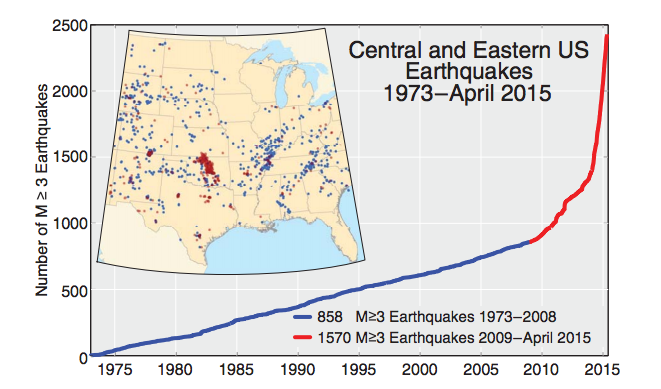
\includegraphics[width=0.7\textwidth]{induced}
   \caption{\label{inducedfig} From \cite{seis_induced}. Count of M $\geq3$ earthquakes in the central and eastern United States from 1973 to April 2015. Two abrupt increases in the earthquake rate occurred in 2009 and 2013. Red dots represent earthquakes that occurred between 2009 and April 2015, and blue dots represent earthquakes that occurred between 1973 and 2008. Prior to 2009, earthquakes were spread across the United States. Beginning in 2009 the earthquakes are tightly clustered in a few areas.}
\end{figure}

The data used for enumerating this dimension of each well was the "Quaternary Fault and Fold Database of the United States," provided by the U.S. Geological Service. The data base included the shape and geographical positioning of each fault in the U.S. as well as the slip rate, a measure of the activity of the fault. Following the same logic in (1) lead me to the formula 
$$score(n_i) =  \mathbb{E}\bigg[\sum_{j=0}^k \frac{s_j}{dist^2(n_i, r_j)}\bigg]$$
where $s_j$ here is the slip rate of the $j$th fault and $dist(n_i, r_j)$ is the distance between the $i$th injection site and the nearest point to it on the $j$th fault line. 

\item \emph{Proximity to and Size of Population Centers} A major concern with many drilling projects is public acceptance. It doesn't matter how great of a resource Manhattan could hypothetically be sitting on top of, carbon won't be stored under it any time soon. With any \emph{perceived} potential risk this might have to the surrounding area, a population, especially a large population, is likely to be slow to accept and approve the project. In the current zeitgeist, it is likely that 2 million people would prefer to have a few more tons in the atmosphere than sitting under their homes. The importance of a potential injection site's relationship to a population center is discussed in \cite{seis_induced} and is certainly an important aspect of the viability of any potential site. 

The scoring for this dimension is based on data from the U.S. Census Beareu. Each of the 500 U.S. cities with the largest populations were listed with their populations and geographical coordinates. Similar logic was applied to scoring potential injection sites with respect to this dimension as was applied to the above dimension. However, in this instance we have $s_j$ as the total population of the $j$th city. This again gives,
$$score(n_i) =  \mathbb{E}\bigg[\sum_{j=0}^k \frac{s_j}{dist^2(n_i, r_j)}\bigg]$$


\item \emph{Proximity to National Parks} While the immediate threat to human life is lower than that of a city, the public or governmental acceptance of performing an injection under or near a National Park or Federally protected land must be considered in tandem with the viability of a potential site. This is motivated by the same reasoning discussed in the above three items.

To score National Parks, I set $s_j = 1 \forall j$ to avoid making value judgements about the importance of different parks. Here, the function $dist(n_i, r_j)$ is the distance between the geographical center of a park $r_j$ and injection site $n_i$.
$$score(n_i) =  \mathbb{E}\bigg[\sum_{j=0}^k \frac{s_j = 1}{dist^2(n_i, r_j)}\bigg]$$

\end{enumerate} 

\subsection{Fuzzy c-Means Clustering}\label{fuzz}
So that this paper can be self contained, I include an introduction to Fuzzy c-Means clustering and related concepts. This section will consist of an introduction to clustering followed by the way in which it is applied to this work.

\subsubsection{Introduction to Fuzzy c-Means Clustering}
\par In general, clustering is an analysis in machine learning theory that takes in $x$ data elements and outputs a set of $k$ buckets, where each element, $x_i$ belongs to exactly one bucket, $k_j$. The goal here is for the algorithm to halt in the state such that $\forall k_j, k_j = \{$most similar items$\}$, where $\|k_j\|$ is not necessarily the same for any two buckets. From this the question arises, what does \emph{similar} mean? This definition will be the deciding factor in how we determine the elements of our $k$ buckets.   

\par There are many different notions of \emph{similar} in clustering theory, but the most applicable to be discussed here is that of centroid-based clustering. In centroid-based clustering, the goal is to find $k$ central vectors that minimize the sum-squared distances to each of the $\leq j$ vectors that they contain. Fuzzy Clustering, deriving its name from Fuzzy Logic as published by Columbia alumnus Lotfi Zadeh in the 1960s, is the paradigm under which each of the $j$ objects in the data set has a degree of membership (a sum squared distance) to each of the $k$ centers. In traditional $k$-means Clustering, each of the $j$ objects distance with respect to only one center would be minimized. Though this form of clustering is much better studied than Fuzzy c-Means, it is not as suitable to this application because there is a lot of value to be had in minimizing membership to each of the $k$ clusters, rather than maximizing membership to one of them, to be further discussed in the next section.  
\emph{N.B.} For more detailed information on Fuzzy c-Means clustering and the implementation of the algorithm employed by this paper see \cite{cmeanspaper}. 

\subsubsection{Application of Fuzzy c-Means Clustering} 
\par The choice of Fuzzy c-Means clustering follows from the idea that the factors that define the viability of a formation in many cases, especially with respect to those features isolated for this work, is defined by the risks associated with injection into that site. In terms of Fuzzy c-Means clustering, we can think therefore think about sites that incur the most risk in terms of their membership coefficient to the subset of the $k$ clusters that reflect risk.\footnote{This section assumes the construction of the vectors as described in Section \ref{wellchar}}. Since we in fact want to mitigate this risk, the subset of the $j$ formations that have the lowest membership coefficients with respect to the negative risk centers will be deemed the potential injection sites with the least relevant risk.

\par Further motivating the choice of a Fuzzy clustering algorithm is that the purpose of this work is not to only prescribe which potential sites are best for injection, but more importantly to create a model that will allow people in the field to make this conjecture based on the tool's analysis. In discovering membership coefficients of each potential site with respect to each cluster center, a Fuzzy clustering analysis provides significantly more information to make a decision off of. For example, this Fuzzy clustering model of the data will allow for queries given a certain threshold tolerance for potential impact on a water source and a certain minimum capacity of storage that the mode. Further, based on the success of previously completed saline injection projects we can discover potential sites with similar properties because in its nature this Fuzzy cluster based model immediately clusters like vectors (representations of formations) together. Thus, we can plot vectors representing already existing projects and see what other sites are clustered with them to prescribe sites for future injection. 

%\subsection{Analysis of Sites Already in Use}
%Talk about the few points that represent wells that are already in use and how they fit in your model. 


\section{Results}
Unfortunately, there are no deterministic algorithms that exist to compute the $k$ Fuzzy c-Means clusters from a set of $j$ vectors exactly. For that reason we apply the FPC algorithm cited in Section \ref{fuzz} to approximate the centers of the clustering analysis. Furthermore, since this algorithm requires a predefined $k$, we run the FPC algorithm for $k \in [5,11]$, as it is correct practice to reduce the dimensionality of the data set (in this case $k < 12$) when clustering the $j$ vectors around $k$ centers. Figures \ref{clusterfig} and \ref {k_means_sil} show the graphical results of the clusterings. For exact numerical results regarding the found cluster centers, see the tables in Appendix A. 

\begin{figure}[H]
\centering
\caption{\label{clusterfig} Each Figure (a - e) shows the clusters resulting from the running of the FPC algorithm for unique values if $k$. These results actually occur in 9-dimensional space, so a 6 degree Principal Component Analysis was used to reduce the dimensionality of each vector to 3 so that they could be pictured in these figures. For this reason, some of the detail gets lost, but the clusters are all still discernable. In Section \ref{danda} we will find (d), where $k = 9$, to be the preferred clustering analysis, hence it is colored differently than the rest of the plots.}
\begin{tabular}{cc}
  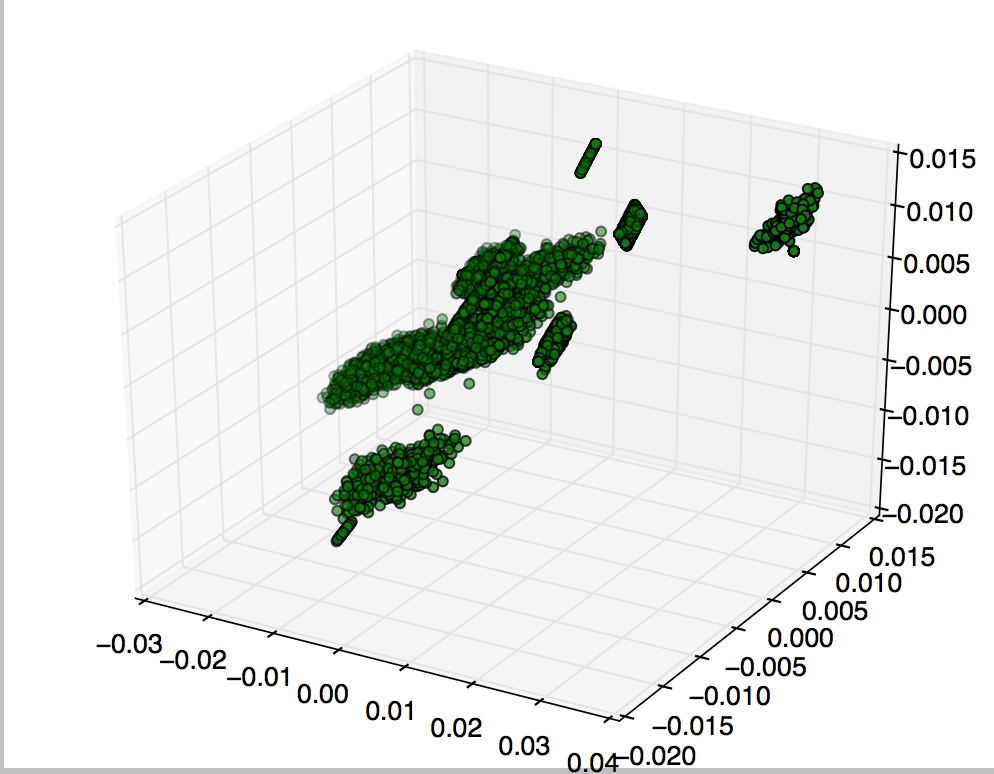
\includegraphics[width=65mm]{k5} &   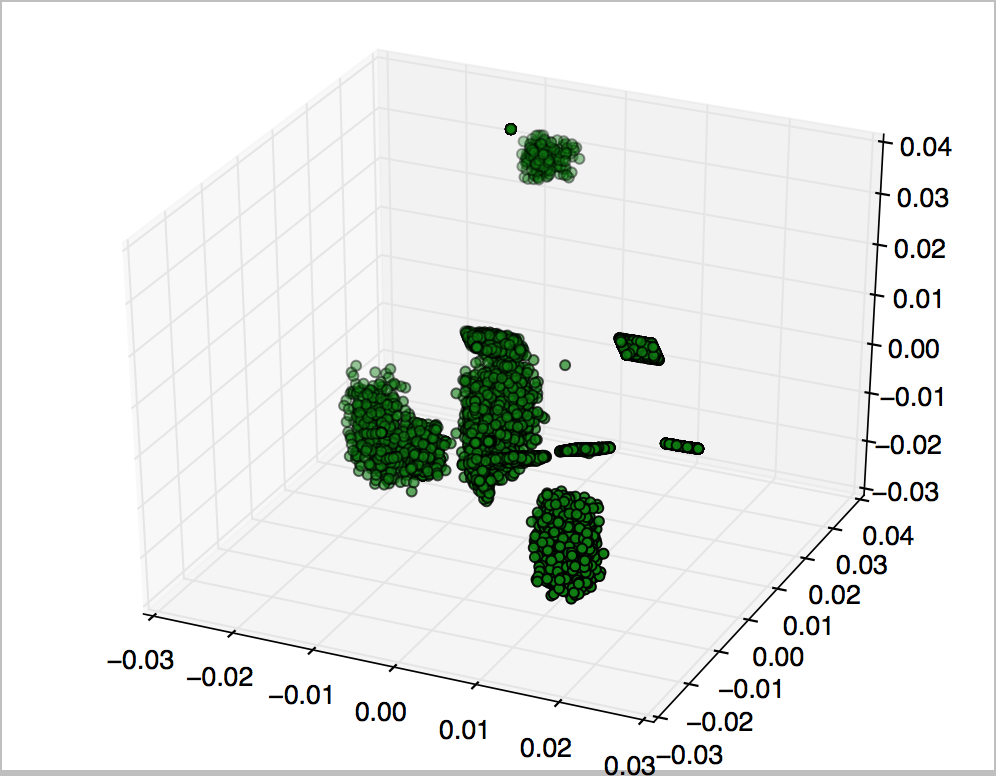
\includegraphics[width=65mm]{k6} \\
(a) $k = 5, FPC = 0.6667$ & (b) $k = 6, FPC = .8333$ \\[6pt]
 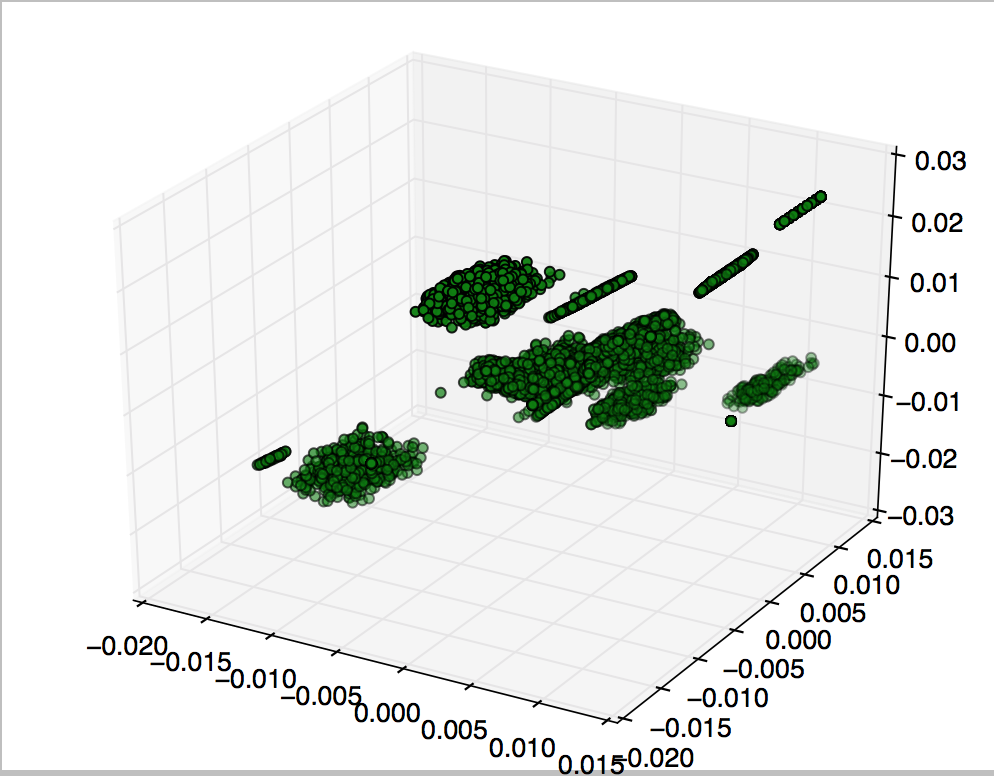
\includegraphics[width=65mm]{k7} &   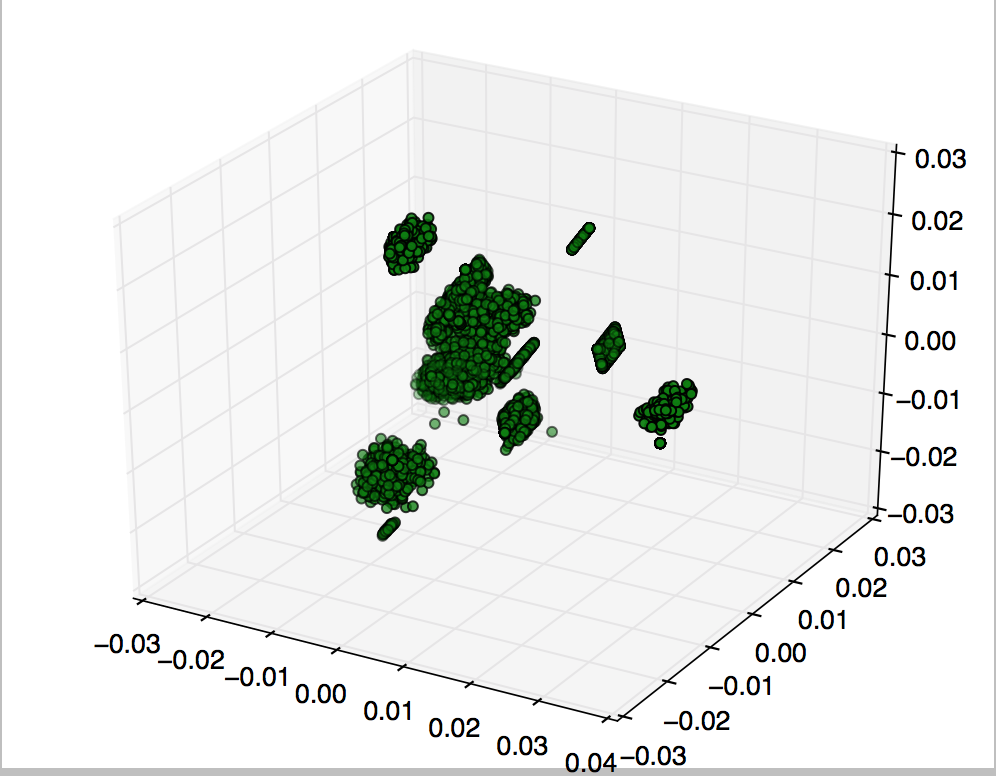
\includegraphics[width=65mm]{k8} \\
(c) $k = 7, FPC = .8333$ & (d) $k = 8, FPC =  0.6667$ \\[6pt]
\end{tabular}
\end{figure}
\begin{figure}[H]
\centering
\begin{tabular}{cc}
 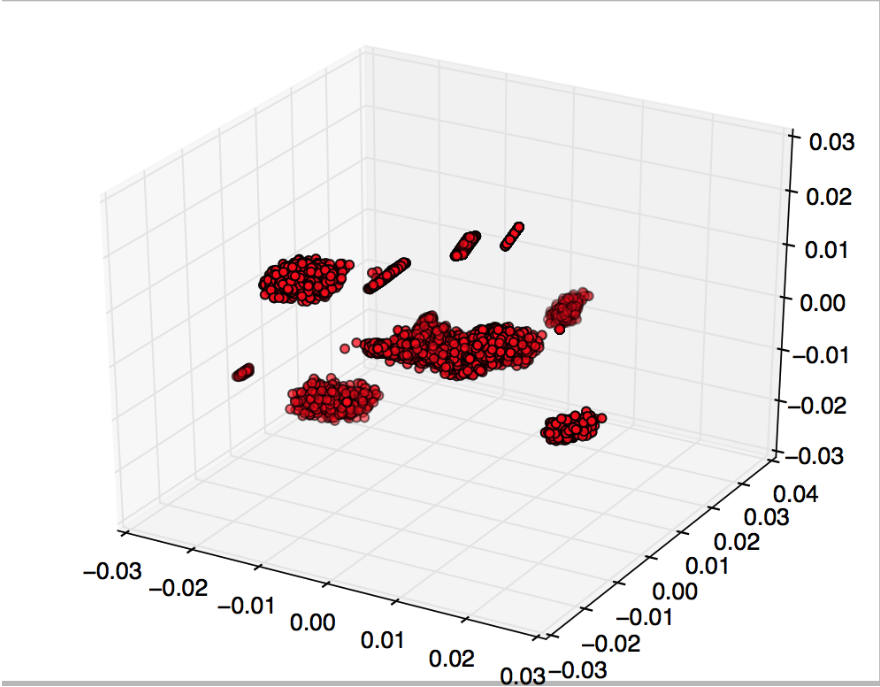
\includegraphics[width=65mm]{k9} &   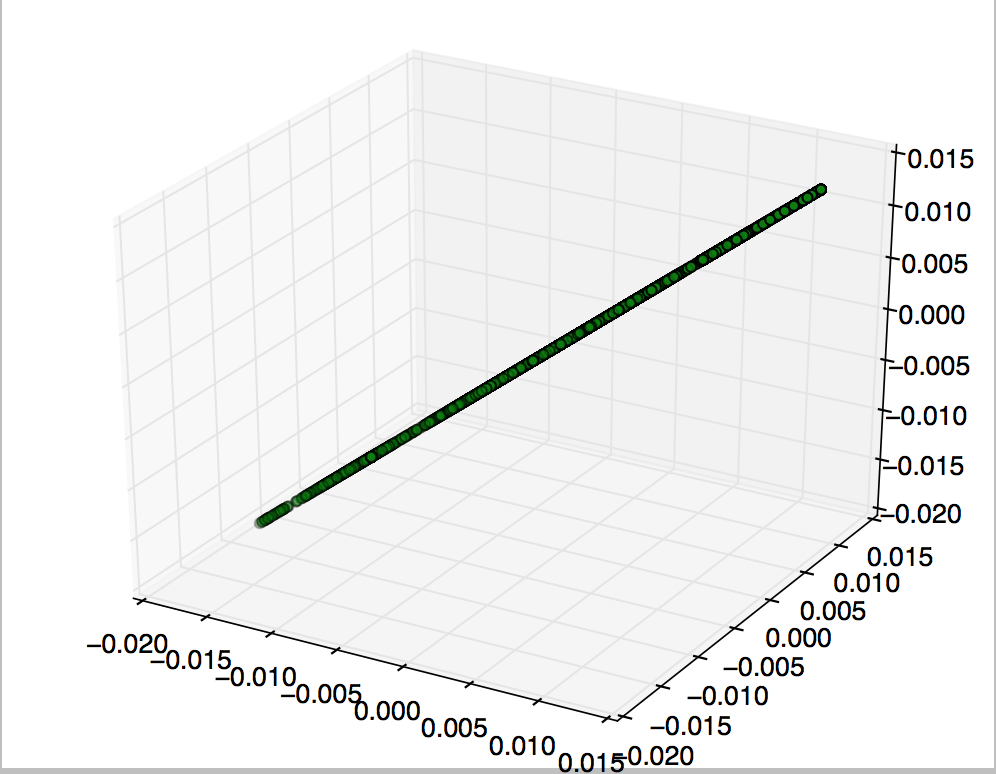
\includegraphics[width=65mm]{k10} \\
(d) $k = 9, FPC = .6111$ & (e) $k = 10, FPC = 1$ \\[6pt]
\end{tabular}
\end{figure}

\begin{figure}[H]%this figure will be at the right
   \centering
   \caption{\label{k_means_sil} This is a silhouette plot evaluating the fit of the model to the data. It is a common method of evaluation used in addition to the FPC. This plot shows the silhouette values for each value of $k$. Note that the cluster values range from $[2,7]$. These are offset by $-3$ so a cluster value of 5 on the chart shows $k = 5 + 3 = 8$. In general, the closer the silhouette value is to 1, the better the fit of the model. }
  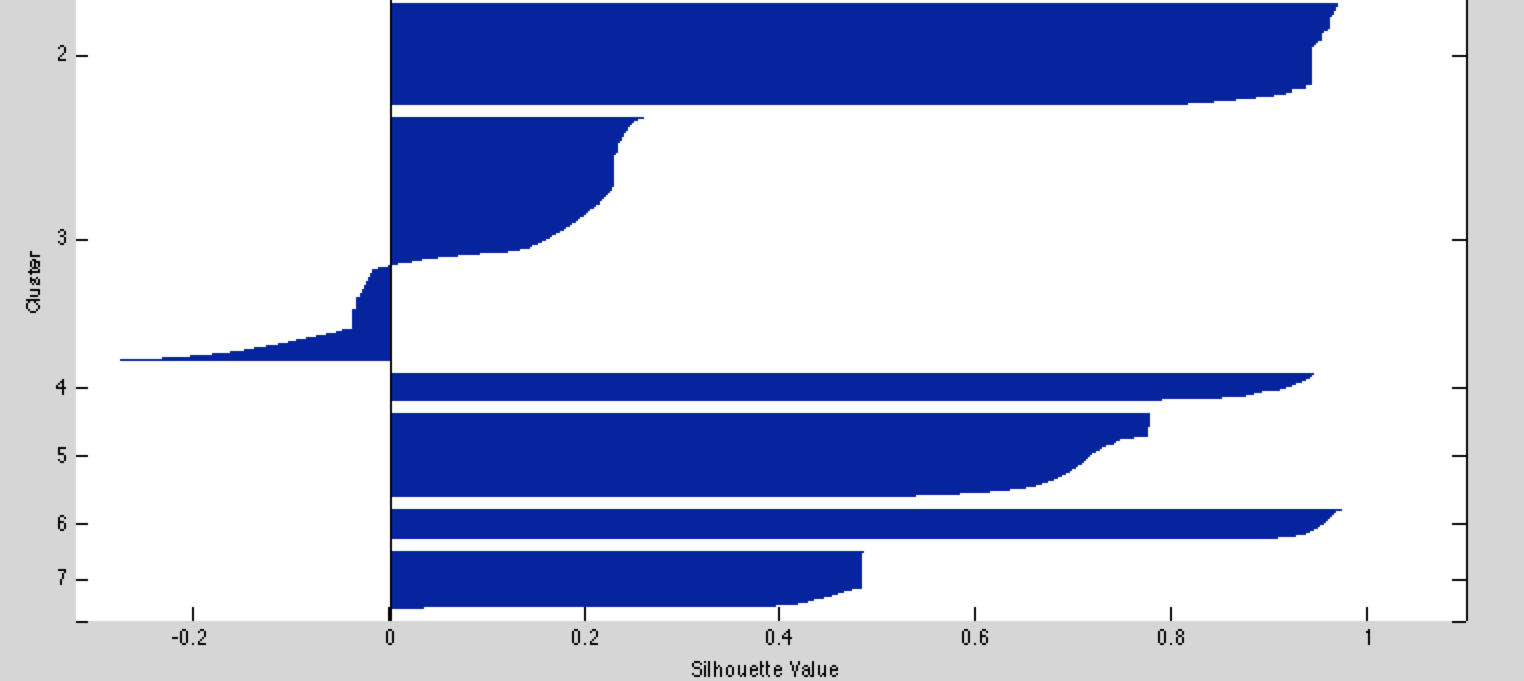
\includegraphics[width=0.75\textwidth]{k_means_sil}
\end{figure}

\section{Discussion and Analysis}\label{danda}
\subsection{Fuzzy Clustering Results}\label{fcmr}
Before we discuss the resulting model's implications for analysis of potential carbon storage sites, we must select one of the model's presented in Figure \ref{clusterfig} as the best model. 
The partition coefficient (FPC) will be important in choosing our preferred model. In discussing the partition coefficient following in the work of \cite{dunnbar} writing $FPC = \frac{1}{N}\sum_{k = 1}^k \sum_{i = 1}^N m_{ik}^2$. From this definition of the partitioning coefficient we find that $FPC = \frac{1}{k}$, when a given vector $j$ belongs equally to all $k$ clusters and that $FPC = 1$ when $j_{k_i} = 1$ for a unique value of $i$ and $j_{k_i} = 0$ for all other values of $i$, such that $i \in [1, k]$. Now given $FPC \in [\frac{1}{k}, 1]$ we set an optimal value of $FPC_k = avg(\frac{1}{k}, 1) =  \frac{1+k}{2k}$. 
Originally, the clustering algorithm was to be run $\forall k \in [5,11]$. As per Figure \ref{clusterfig}, this was resolved to a maximum value of $k = 10$ because at $k = 10$ we see $FPC_{10} = 1$. In examining $k = 9$, we find that $FPC_9 = \frac{10}{18} \approx \frac{11}{18}$, the optimal value of $FPC$ for $k = 9$. For all $k$, this is the closest value of $FPC_k$ to the optimal value of $FPC_k$, which immediately makes the clustering analysis for $k = 9$ the favorable choice. To further justify the choice of the clustering model of $k = 9$, we look to the silhouette diagram in Figure \ref{k_means_sil}. As touched on in Figure \ref{k_means_sil}, the better the fit of the model, the closer the silhouette value is to 1. We find this occurs near $k = 5, 7, 9$. With $k = 9$ deemed a good fit by the silhouette analysis as well, we comfortably select the clustering analysis around 9 centers as the best model for the data. 

\subsection{Translating \ref{fcmr} to Insight on Saline Formations} 
\begin{wrapfigure}{R}{.65\linewidth}
\centering
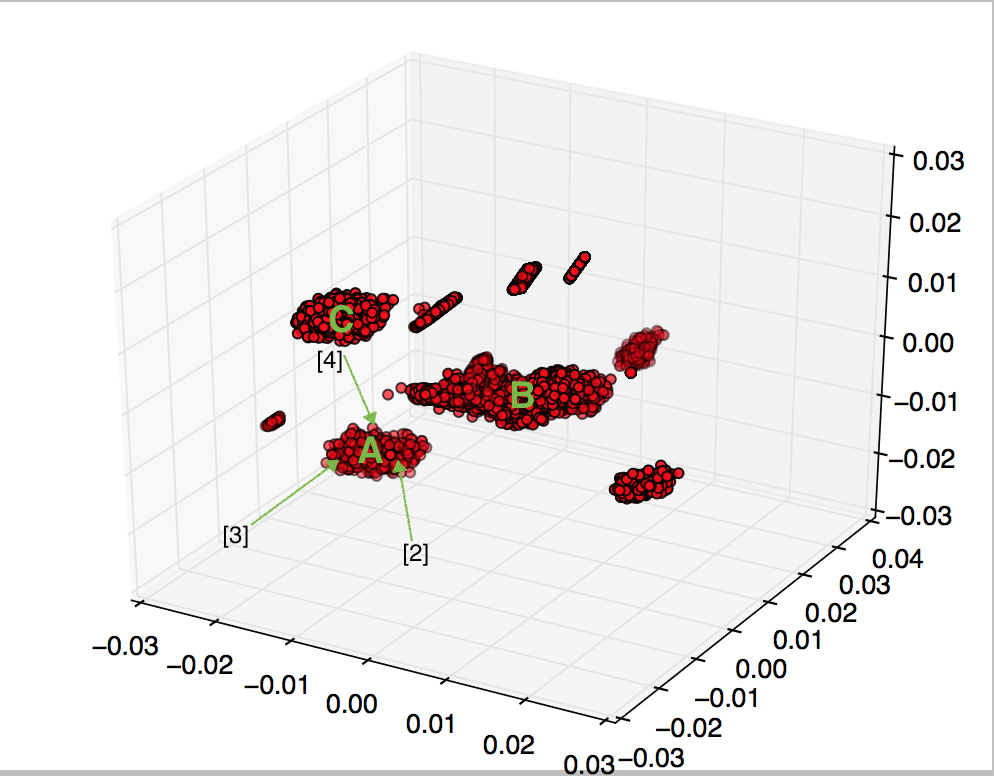
\includegraphics[width=.65\linewidth]{k9disc}
\caption{\label{k99disc} A reproduction of Figure \ref{clusterfig}(d) overlayed with pointers to the points representing the formations being used in \cite{midwestinject}, \cite{midwestinject2}, \cite{southeastinject}. Being that there are 180,000 points (one for each formation in the database) it is impossible to see these points directly, as they're covered by other points in their cluster.}
\end{wrapfigure}

\par Now that we have a reasonable model for the general similarity of saline formations as well as the relationship between different features of the formations, we can apply the findings to conjecturing some of the best potential injection sites in the U.S. To begin, let's consider the saline injection projects in \cite{midwestinject}, \cite{midwestinject2}, \cite{southeastinject}. As we see in Figure \ref{fcmr}, all three of the formations used in these projects exist in the same cluster. This is a fascinating result because the model groups these formations, which were each investigated for $3+$ years before an injection was approved, together as similar based on their characteristics. For this reason, we focus our study on this cluster, cluster $A$, to discover more potentially viable injection sites. Cluster $A$ contains about 22,000 sites $\approx 12\%$ of the saline formation injection sites in the database listed by NATCARB. This makes it the third largest cluster, behind clusters $B$ and $C$ as per Figure \ref{k99disc}, with $\|B\| \approx 56\%$ and $\|C\| \approx 16\%$. \footnote{22,000 sites is far beyond what can be listed in the forum of this paper, but pulling the code down from the hosted repository listed earlier, this list can be exactly reproduced. I am actively working on a way to make such a large list useful. My current method involves reducing the list of 22,000 to a smaller list of groups that contain geographically proximate sites.} 

\par Upon inspection, it is difficult to isolate exactly the dimensions and thresholds that gain a site entry into cluster $A$. However, the dimensions that are prevalent in $B$ and $C$ allow is to form something of a negative definition of $A$. 
(You should discuss this more.......)

\section{Future Work}
\subsection{Isolating Better Heuristics for Scoring Formation Dimensions}
This is the aspect of this project that I would like to develop into a tool for people that actively work on this problem. The clustering algorithm depends immediately upon every dimension of each component vector, and scoring the importance and risk involved with each scored dimension (fault line, population, national park and water source proximity). Thus, for every different method of scoring, different clusters will result. While I am able to develop heuristics, it is much more powerful for people in industries and academia that work on this problem to be able to parameterize their judgements of the weights of different characteristics of a formation and other values and have the ability to rapidly test their hypotheses against unique models. This is where the real beauty of this work lies and is the most immediate item I am working on. 

\subsection{Better Characterization of Saline Formations}\label{betterchar}
The 12 features isolated for characterization are a minimal set for reasonable characterization of saline formations. Better and more detailed (higher dimensional) characterizations of these formations would necessarily allow for more data for Fuzzy c-Means clustering to base its similarity measures on, thereby increasing the accuracy and effectiveness of this tool. Further dimensions include the existence of a caprock over the layer of porous rock. The existence of such a caprock is extremely important to the viability of a potential site as it plays an important part in keeping the injected carbon below the surface and in place. I would like to further investigate and apply some of the findings of \cite{natcarb_risk} and \cite{PredRisk2013} in order to represent every formation by the most relevantly detailed dimensions possible. 

\subsection{Finding a Better Definition of Each Cluster}
One of the paramount benefits of machine learning techniques like the Fuzzy c-Means algorithm is that it has the ability to recognize and act on patterns that humans can not possibly identify. For this reason, there are tremendous insights that lay in the way that each cluster is defined and characterized. 
This is an extremely difficult problem, but I believe that an analysis of the vectors contained in each cluster could yield insights much deeper than the mere inspections given here. By applying the Fuzzy c-Means algorithm to each cluster independently, especially cluster $A$, could allow us to gain a better understanding of the amalgam of characteristics that define each cluster by further isolating the dimensions of the sites contained in them. 

\section{Conclusion}

Value judgements -- who is to say how imporatant it is to not do this under a national park, etc- --- this system allows for quick hypotheses testing based on different criteria, on different values and best of all can isolate some that meet everyones turf the best, givingbetter information of better options 
 
\begin{thebibliography}{9}

\bibitem{QuantRiskS2014}
Wriedt, J., Deo, M., Han, W. S., and Lepinski, J.
\textit{A methodology for quantifying risk and likelihood of failure for carbon dioxide injection into deep saline reservoirs}
International Journal of Greenhouse Gas Control 20 (2014), 196-211.

\bibitem{midwestinject}
Albenze, Erik, and Sallie Greenberg. 
\textit{Midwest Geological Sequestration Consortium $\|$ Development Phase}
National Energy Technology Laboratory, 1 Nov. 2015. http://www.netl.doe.gov/publications/factsheets/project/NT42588.pdf.

\bibitem{midwestinject2}
McNemar, Andrea, and Neeraj Gupta. 
\textit{Midwest Regional Carbon Sequestration Partnership $\|$ Development Phase}
National Energy Technology Laboratory, 1 Nov. 2015. http://www.netl.doe.gov/publications/factsheets/project/NT42589.pdf.

\bibitem{southeastinject}
Brown, Bruce, and Ken Nemeth. 
\textit{Southeast Regional Carbon Sequestration Partnership $\|$ Validation Phase}
National Energy Technology Laboratory, 1 Dec. 2012. http://www.netl.doe.gov/publications/factsheets/project/NT42590-P2.pdf.

\bibitem{whysaline}
\textit{Carbon Storage R\&D} Department of Energy. Office of Fossil Energy. Web. 01 May 2016.

\bibitem{atlas}
Friedmann, S. 
\textit{Carbon Storage Atlas V} 
National Energy Technology Laboratory, 1 Aug 2015.

\bibitem{natcarb_risk}
\textit{Carbon Storage Technology Program Plan}
Clean Coal Research Program, Department of Energy. Office of Fossil Energy. 1 Dec. 2014.

\bibitem{seis_induced}
Rubinstein, Justin L., Mahani, Alireza B.
\textit{Myths and Facts on Wastewater Injection, Hydraulic Fracturing, Enhanced Oil Recovery, and Induced Seismicity}
Seismological Research Letters 86, 4 (2015), 1-8. 

\bibitem{PredRisk2013}
Balashov, Victor N., et al.
\textit{Predictive modeling of CO 2 sequestration in deep saline sandstone reservoirs: impacts of geochemical kinetics}
Applied geochemistry 30 (2013): 41-56.

\bibitem{cmeanspaper}
Bezdek, James C., Robert Ehrlich, and William Full.
\textit{FCM: The fuzzy c-means clustering algorithm}
Computers and Geosciences 10.2 (1984): 191-203.

\bibitem{dunnbar}
Trauwaert, E. 
\textit{On the meaning of Dunn's partition coefficient for fuzzy clusters}
Fuzzy sets and systems 25.2 (1988): 217-242.

\end{thebibliography}

\pagebreak
\section{Appendix A}
These tables compliment the results in Figure \ref{clusterfig}. The tables list the 9-dimensional coordinates of the centers approximated by each run of the Fuzzy c-Means clustering algorithm for $k \in [5,10]$. Note that these centers were originally 12 dimensions (one for each dimension of the feature vectors), but were dimensionally reduced with Principal Component Analysis to reduce the complexity of the computations without loss of generality. 

\begin{table}[h]
\centering
\caption{9 dimensional coordinates of the centers found at each run of Fuzzy c-Means clustering.}
\label{tablecenters}
\begin{tabular}{lllllllll}
k = 5   & fpc =   & 0.6667  &         &         &         &         &         &         \\
0.0015  & -0.0025 & 0.0086  & -0.0107 & -0.0009 & 0.0066  & -0.0126 & 0.0017  & 0.0083  \\
-0.0107 & -0.0027 & -0.0038 & 0.0017  & 0.0092  & -0.0004 & 0.0225  & -0.0067 & 0.0081  \\
-0.0083 & 0.0084  & 0.0036  & -0.0016 & -0.0015 & 0.0086  & -0.0107 & -0.0009 & 0.0066  \\
-0.0052 & 0.0017  & 0.0083  & -0.0107 & -0.0027 & -0.0019 & 0.0017  & 0.0101  & 0.0007  \\
0.0224  & -0.0067 & 0.0081  & -0.0051 & 0.0085  & -0.0140 & 0.0036  & -0.0019 & 0.0086  \\
        &         &         &         &         &         &         &         &         \\
k = 6   & fpc =   & 0.8333  &         &         &         &         &         &         \\
-0.0006 & 0.0069  & 0.0027  & -0.0092 & 0.0071  & 0.0013  & -0.0035 & 0.0082  & 0.0026  \\
-0.0092 & 0.0065  & -0.0032 & 0.0082  & 0.0029  & 0.0086  & 0.0031  & -0.0015 & 0.0028  \\
-0.0007 & 0.0015  & 0.0098  & -0.0025 & 0.0077  & 0.0027  & -0.0092 & 0.0071  & 0.0013  \\
0.0009  & 0.0082  & 0.0026  & -0.0092 & 0.0065  & -0.0016 & 0.0082  & 0.0027  & 0.0089  \\
0.0029  & -0.0015 & 0.0030  & 0.0020  & 0.0019  & -0.0050 & 0.0007  & 0.0074  & 0.0027  \\
-0.0092 & 0.0071  & 0.0013  & -0.0039 & 0.0082  & 0.0026  & -0.0092 & 0.0065  & -0.0017 \\

        &         &         &         &         &         &         &         &         \\
k = 7   & fpc =   & 0.8333  &         &         &         &         &         &         \\
0.0015  & -0.0025 & 0.0086  & -0.0107 & -0.0009 & 0.0066  & -0.0126 & 0.0017  & 0.0083  \\
-0.0107 & -0.0027 & -0.0038 & 0.0017  & 0.0092  & -0.0004 & 0.0225  & -0.0067 & 0.0081  \\
-0.0083 & 0.0084  & 0.0036  & -0.0016 & -0.0015 & 0.0086  & -0.0107 & -0.0009 & 0.0066  \\
-0.0052 & 0.0017  & 0.0083  & -0.0107 & -0.0027 & -0.0019 & 0.0017  & 0.0101  & 0.0007  \\
0.0224  & -0.0067 & 0.0081  & -0.0051 & 0.0085  & -0.0140 & 0.0036  & -0.0019 & 0.0086  \\
-0.0107 & -0.0009 & 0.0066  & -0.0118 & 0.0017  & 0.0083  & -0.0107 & -0.0027 & -0.0024 \\
0.0017  & 0.0104  & -0.0021 & 0.0236  & -0.0063 & 0.0089  & -0.0049 & 0.0077  & -0.0126 \\
\end{tabular}
\end{table}
\begin{table}[]
\begin{tabular}{lllllllll}
k = 8   & fpc =   & 0.6667  &         &         &         &         &         &         \\
-0.0006 & 0.0069  & 0.0027  & -0.0092 & 0.0071  & 0.0013  & -0.0035 & 0.0082  & 0.0026  \\
-0.0092 & 0.0065  & -0.0032 & 0.0082  & 0.0029  & 0.0086  & 0.0031  & -0.0015 & 0.0028  \\
-0.0007 & 0.0015  & 0.0098  & -0.0025 & 0.0077  & 0.0027  & -0.0092 & 0.0071  & 0.0013  \\
0.0009  & 0.0082  & 0.0026  & -0.0092 & 0.0065  & -0.0016 & 0.0082  & 0.0027  & 0.0089  \\
0.0029  & -0.0015 & 0.0030  & 0.0020  & 0.0019  & -0.0050 & 0.0007  & 0.0074  & 0.0027  \\
-0.0092 & 0.0071  & 0.0013  & -0.0039 & 0.0082  & 0.0026  & -0.0092 & 0.0065  & -0.0017 \\
0.0082  & 0.0030  & 0.0072  & 0.0044  & -0.0011 & 0.0042  & 0.0022  & 0.0010  & -0.0047 \\
0.0011  & 0.0081  & 0.0035  & -0.0086 & 0.0067  & 0.0013  & -0.0041 & 0.0079  & 0.0026  \\
        &         &         &         &         &         &         &         &         \\
k = 9   & fpc =   & 0.6111  &         &         &         &         &         &         \\
0.0015  & -0.0025 & 0.0086  & -0.0107 & -0.0009 & 0.0066  & -0.0126 & 0.0017  & 0.0083  \\
-0.0107 & -0.0027 & -0.0038 & 0.0017  & 0.0092  & -0.0004 & 0.0225  & -0.0067 & 0.0081  \\
-0.0083 & 0.0084  & 0.0036  & -0.0016 & -0.0015 & 0.0086  & -0.0107 & -0.0009 & 0.0066  \\
-0.0052 & 0.0017  & 0.0083  & -0.0107 & -0.0027 & -0.0019 & 0.0017  & 0.0101  & 0.0007  \\
0.0224  & -0.0067 & 0.0081  & -0.0051 & 0.0085  & -0.0140 & 0.0036  & -0.0019 & 0.0086  \\
-0.0107 & -0.0009 & 0.0066  & -0.0118 & 0.0017  & 0.0083  & -0.0107 & -0.0027 & -0.0024 \\
0.0017  & 0.0104  & -0.0021 & 0.0236  & -0.0063 & 0.0089  & -0.0049 & 0.0077  & -0.0126 \\
0.0036  & -0.0011 & 0.0102  & -0.0106 & -0.0020 & 0.0066  & -0.0120 & -0.0001 & 0.0083  \\
-0.0107 & -0.0027 & -0.0028 & 0.0041  & 0.0099  & -0.0009 & 0.0222  & -0.0067 & 0.0084  \\
        &         &         &         &         &         &         &         &         \\
k = 10  & fpc=    & 1.0000  &         &         &         &         &         &         \\
-0.0005 & 0.0114  & 0.0039  & -0.0123 & 0.0122  & 0.0004  & 0.0172  & -0.0116 & 0.0040  \\
-0.0123 & 0.0108  & 0.0000  & -0.0116 & 0.0039  & 0.0150  & -0.0071 & -0.0053 & 0.0028  \\
0.0090  & 0.0013  & -0.0054 & -0.0014 & 0.0131  & 0.0039  & -0.0123 & 0.0122  & 0.0004  \\
-0.0006 & -0.0116 & 0.0039  & -0.0123 & 0.0108  & -0.0011 & -0.0116 & 0.0029  & 0.0158  \\
-0.0056 & -0.0053 & -0.0010 & 0.0130  & 0.0023  & 0.0137  & 0.0008  & 0.0125  & 0.0039  \\
-0.0123 & 0.0122  & 0.0004  & 0.0176  & -0.0116 & 0.0039  & -0.0123 & 0.0108  & -0.0013 \\
-0.0116 & 0.0033  & 0.0120  & -0.0063 & -0.0044 & 0.0003  & 0.0132  & 0.0007  & 0.0133  \\
-0.0013 & 0.0139  & 0.0047  & -0.0115 & 0.0113  & 0.0004  & 0.0170  & 0.0139  & 0.0039  \\
0.0108  & -0.0019 & -0.0087 & 0.0053  & 0.0122  & -0.0061 & -0.0053 & -0.0012 & 0.0108  \\
0.0015  & 0.0132  & 0.0003  & 0.0126  & 0.0039  & -0.0123 & 0.0122  & 0.0004  & 0.0138 
\end{tabular}
\end{table}
\end{document}
